\chapter{Deep integrations on polarization with PAPER-128}
\label{chapter:eor_window_psa128}

In Chapter~\ref{chapter:eor_window_paper32img}, I presented polarized power spectra from a short integration -- a few hours of one night -- over a wide range of $k_{\perp}$-modes probed by the PAPER-32 polarized imaging array \citep{Kohn.16}. Chapter~\ref{chapter:eor_window_HERA} presented the first power spectral results from HERA. The HERA-19 commissioning array was small and dense, meaning that only a few $k_{\perp}$-modes were accessible. For that study, we averaged over 10 hours per night, for 8 consecutive nights {\color{red} (Kohn et al. 2018)}. This Chapter presents results from the PAPER-128 array. In this Chapter I present roughly one quarter of the total number of observations recorded by this interferometer (Section~\ref{sec:psa128_obs}). I show results of a deep integration on a very narrow range of $k_{\perp}$-modes (corresponding to $\sim$30\,m spacings of the redundant grid; Section~\ref{sec:psa128_results}) and discuss the implications for deep, fully-polarized integrations with large interferometers (Section~\ref{sec:psa128_conc}).

\section{Observations \& Reduction}
\label{sec:psa128_obs}
 
PAPER-128 was the largest build-out of the PAPER experiment. As described in Chapter~\ref{chapter:instruments},  PAPER-128 consisted of 128 antennas, 112 of which were arranged in a redundant grid. An annotated photograph of the array is shown in Figure~\ref{fig:psa128photo}. In this section, I review the PAPER-128 campaign (Section~\ref{subsec:psa128_obs_overview}) and the subsequent reduction of roughly one quarter of the total number of observations (Section~\ref{subsec:psa128_s1e2_reduction}).

\begin{figure}
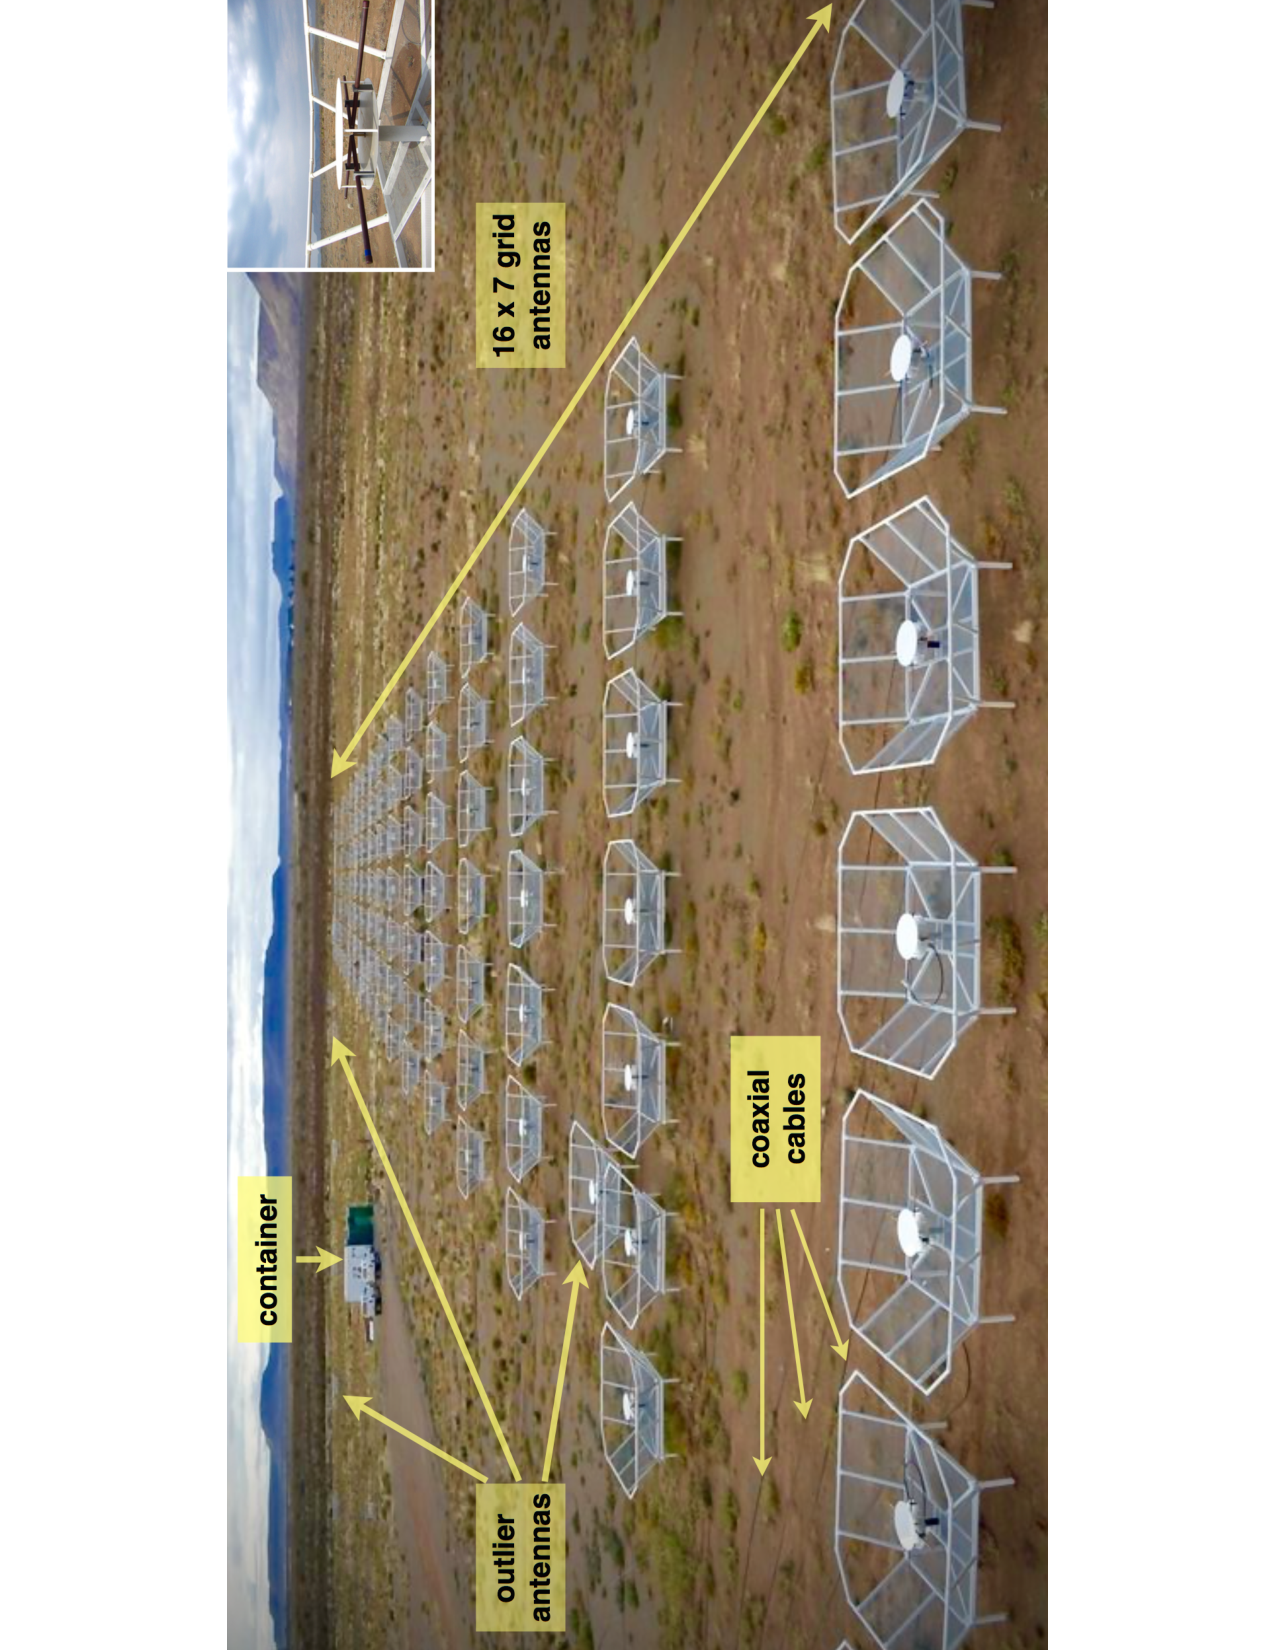
\includegraphics[width=0.8\textwidth, angle=270]{chapters/psa128_pol/figures/array_photo_diagram.pdf}
\caption[An annotated photograph of the PAPER-128 array.]{An annotated photograph of the PAPER-128 array, looking to the East. Highlighted are the 112 antenna redundant grid, with 15\,m East-West spacings between each row; outlier antennas from the main grid used to increase \textit{uv}-coverage; coaxial cables running to the receiverators and correlator (see Chapter~\ref{chapter:instruments}). An inset panel shows a PAPER sleeved dipole. Photo credit: J. E. Aguirre. Figure credit: C. D. Nunhokee; \citep{Nunhokee_thesis}.}
\label{fig:psa128photo}
\end{figure}

\subsection{Overview of PAPER-128 observations}
\label{subsec:psa128_obs_overview}
Observations were recorded for two years, with first light on November 20th 2013 and final readings on January 27th 2015. However, these observations were not always contiguous. Human errors, experimentation and malfunctioning electronics required the correlator and connected electronics to be turned off and restarted, altering the characteristic phasing and gain scale of the array. Each of these restarts constituted the beginning of a new ``Epoch" of the array which required different quality assurance steps and initial calibration stages. Table~\ref{tab:seasons_psa128} summarizes the length and nature of these Epochs. 

\begin{deluxetable}{lllcl}
\centering
\label{tab:seasons_psa128}
\tablewidth{0pt}
\tablecaption{PAPER-128 Observing Seasons \& Epochs}
\tabletypesize{\footnotesize}
\tablehead{
\colhead{Season} & \colhead{Epoch} & \colhead{Julian Dates} & \colhead{Calendar Dates} & \colhead{Notes} \\
}
\startdata
1 & 1 & 2456617 - 2456673 & Nov 20, 2013 - Jan 15, 2014 & 1/8 F-Engine failure \\
   & 2 & 2456678 - 2456724 & Jan 20, 2014 - Mar 7, 2014 &  \\
2 & 1 & 2456625 - 2456732 & Mar 8, 2014 - Mar 7, 2014 & Too few data \\
   & 2 & 2456843 - 2456873 & Jul 4, 2014 - Aug 3, 2014 & Uninteresting LST range \\
   & 3 & 2456881 - 2456928 & Aug 11, 2014 - Sep 27, 2014 &  Many malfunctioning antennas \\
   & 4 & 2456942 - 2457008 & Oct 11, 2014 - Dec 11, 2014 &  \\
   & 5 & 2457030 - 2457050 & Jan 7, 2015 - Jan 27, 2015 &  Many malfunctioning antennas\\
\enddata
\end{deluxetable}

Figure~\ref{fig:psa128_epochs} illustrates the challenge imposed by the correlator restarts. Epoch changes were characterized by large shifts in the overall phase of visibilities, of course leading to changed magnitudes of the real and imaginary parts of the visibilities recorded. The quality assurance metrics described in Chapter~\ref{chapter:data_prep_and_proc} were sensitive to these changes. Of course, absolute calibration -- that is phasing to the correct point on the sky and scaling the visibilities from arbitrary to physical flux density units -- had to be run separately on individual Epochs.

\begin{figure}
\centering
\includegraphics[width=0.7\textwidth]{chapters/psa128_pol/figures/S2_chan100_hist.pdf}
\includegraphics[width=0.5\textwidth]{chapters/psa128_pol/figures/S2_chan100_phasegrid.pdf}
\caption[The challenge of Epoch changes.]{The challenge of Epoch changes. Shown are all of the Season 2 time samples of the visibilities recorded by the 30\,m baseline between antennas 1 and 4, LSTs 0--5, for only the 150\,MHz frequency bin. The above panel shows a histogram of the real part of the visibilities as a function of LST -- there is a dramatic change in magnitude with respect to LST. Likewise, the lower panel shows the phase of each visibility sample (color axis) as a function of LST (vertical axis) and day of observation (x axis). There are obvious large shifts in phase, which require separate calibration stages.}
\label{fig:psa128_epochs}
\end{figure}

As shown in Table~\ref{tab:seasons_psa128}, Season 2 had a larger number of observed nights than Season 1. However, the analysis of Season 2 was especially challenging due to large numbers of malfunctioning antennas. This may have been due to the antennas ageing past a critical point. Nothing in the array was replaced during build-outs except for the correlator; 32 of the antennas had been out in the desert for 4--5 years (PAPER-32) and another 32 for 3--4 years (PAPER-64). Most of the time, these were the antennas that were identified as malfunctioning.

Season 2 Epoch 4 was relatively well-behaved, and may be analyzed in the future. For this work, we concentrated our analysis on Season 1. Season 1 Epoch 2 was ten days shorter than Season 1 Epoch 1, but Epoch 1 had two major challenges associated with it: a data loss event, and an F-engine failure. Due to human error, Epoch 1 data was deleted and had to be restored and recompressed (see Chapter~\ref{chapter:data_prep_and_proc}). This was almost entirely successful, at the loss of one week's worth of observations. The F-engine failure was more critical. We discovered during out analysis that exactly one eighth of the antennas in the array produced noise-like visibilities with the rest of the array, but normal correlations between one another. These antennas had ``seceded" from the array. They shared the characteristic of all being attached to the same F-engine (of which there were eight; see Figure~\ref{fig:instruments_PAPER_Signal_Chain}). This suggested that there was a clock-offset on that F-engine, resulting in no correlation between the signal from those antennas and those running through the other in-sync F-engines.

This left Season 1 Epoch 2 as the most well-characterized and well-behaved Epoch of PAPER-128 observations, and we focused on this Epoch alone from now on. Cross-polarization metrics identified seven incorrectly-rotated antennas, which were corrected during initial processing. Eight antennas were identified as malfunctioning by mean visibility amplitude metrics, including one of those that was incorrectly-rotated. The state of the array for Season 1 Epoch 2 is summarized in Figure~\ref{fig:s1e2_array}.

\begin{figure}
\includegraphics[width=0.6\textwidth]{chapters/psa128_pol/figures/s1e2_array.png}
\caption[Good, bad and rotated antennas in Season 1 Epoch 2.]{Good, bad (red crosses) and rotated (blue circles) antennas in Season 1 Epoch 2, as identified by the cross-polarization and visibility amplitude metrics defined in Chapter~\ref{chapter:data_prep_and_proc}.}
\label{fig:s1e2_array}
\end{figure}

\subsection{Reduction of Season 1 Epoch 2 data}
\label{subsec:psa128_s1e2_reduction}

After correcting for cross-polarized and malfunctioning antennas, we 

%
%  S1E2: 
% - bad JD identification (slices)?, 
% - xx,yy firstcal (single per epoch), 4pol+minV cal + omnixtalk, bl pull, 
% - linCLEAN, lstbin_{fg,fgsub}
% - (unpolarized) PicA (Jacobs13) CASA cal on lstbin_fg
% - Stokes I FRF on all 4pols of fgsub
%
\section{Results}
\label{sec:psa128_results}

% - not-that-great power spectra

\section{Discussion \& Conclusions}
\label{sec:psa128_conc}
% Pitch to "future work", to end the section
% -- levels predicted for detection of Q,U: Nunhokee, Asad
% -- challenges associated with very long integrations: QUALITY ASSURANCE, instrument stability
% -- ionosphere
